\chapter{Targeted Proteolysis}
\label{chap:tarprot}

The module Targeted Proteolysis is designed to post-process the MS
data acquired during the enzymatic proteolysis of a Target protein by a single
protease. In a typical experimental setup both the protease and the Target protein
are mixed together under various experimental conditions and the peptides generated
during the proteolysis are identified by MS. It is expected that
several control experiments and several replicates of the tested experimental
conditions are performed. The main objective of the module is to identify the peptides
with intensity values that are significantly greater in the replicates of the various
experimental conditions tested than in the replicates of the control experiments
at the chosen significance level.

\section{Definitions}

Before explaining in detail the interface and how does the module work, let's make
clear the meaning of the term Filtered peptide in the context of the Targeted
proteolysis module:

\phantomsection
\begin{itemize}
    \item \textit{Filtered peptide}: a relevant peptide with intensity values in a
    given experimental condition that are significantly higher than the intensity
    values in the control at the chosen significance level.
    \label{par:tarprotPIP}
\end{itemize}

The rest of the definitions in \autoref{sec:limprotDefinitions} are valid for this
module too.

\section{The input files}

The module requires a Data file containing the detected peptides
and a sequence file containing the amino acid sequence of the recombinant protein
used in the study. Both files must follow the guidelines specified in \autoref{sec:dataFile}.
In short, the Data file must have a tabular format with tab separated columns and
the name of the columns are expected as first row. The Sequence file is expected
to contain at least one sequence and to be FASTA formatted. If more than one sequence
is found in the Sequence file the first sequence will be taken as the sequence of
the Recombinant protein and the second sequence will be taken as the sequence of
the Native protein. All other sequences are discarded.

\section{The interface}

The tab of the module Targeted Proteolysis is divided in two regions (\autoref{fig:tarprotTab}).

\begin{figure}[h]
    \centering
    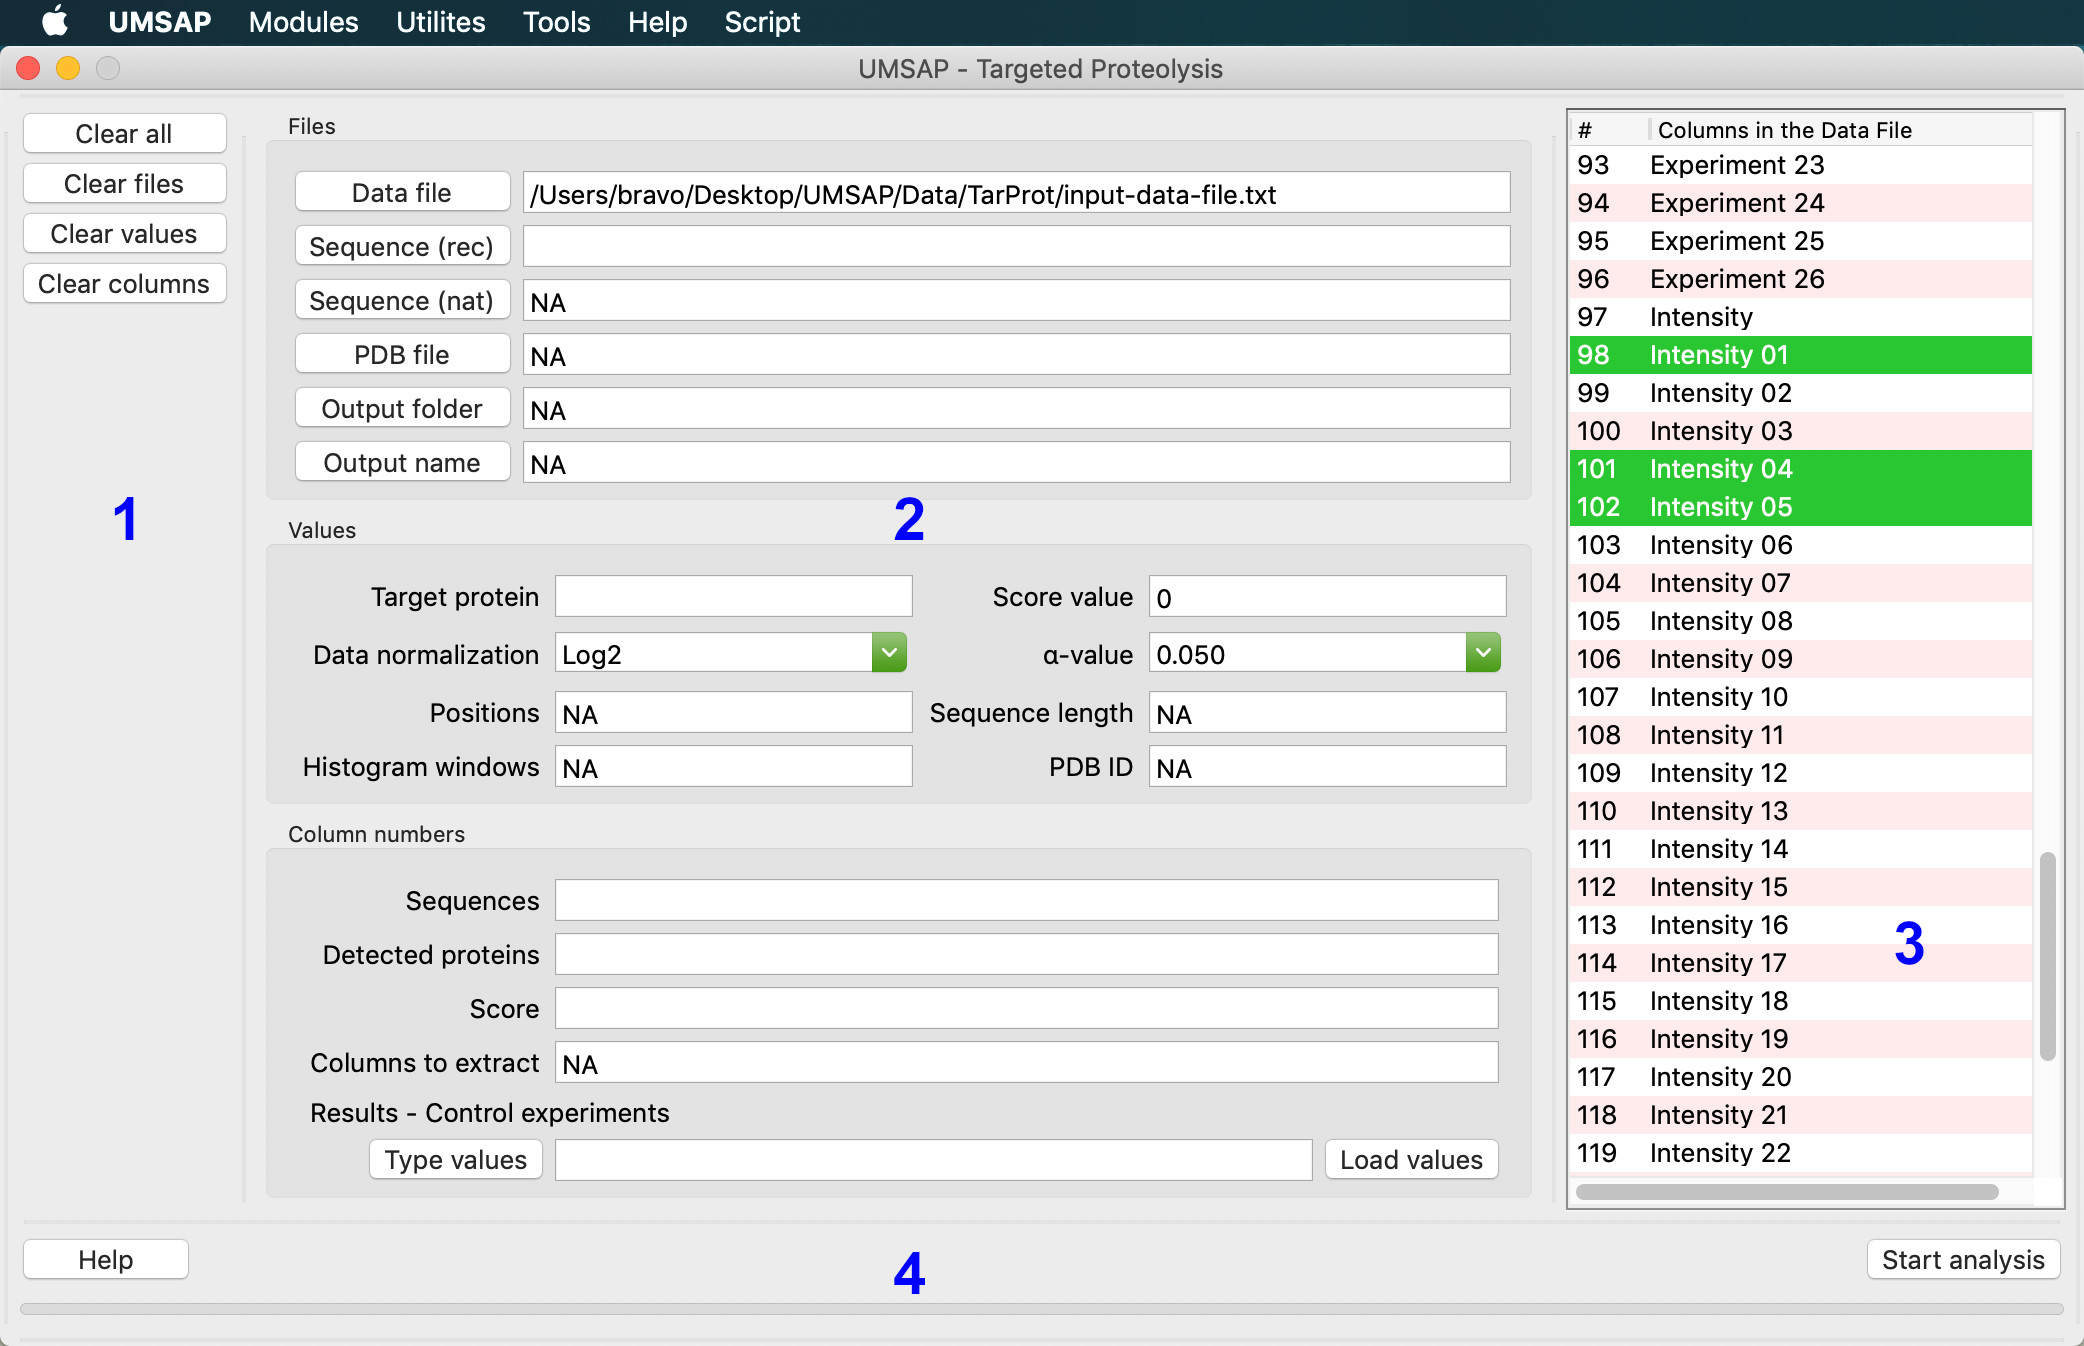
\includegraphics[width=0.7\textwidth]{./IMAGES/MOD-TARPROT/tarprot-mod.jpg}
    \caption[The Targeted Proteolysis module tab]{\textbf{The Targeted Proteolysis
    module tab.} This tab allows performing the analysis of the results obtained
    during an enzymatic proteolysis experiment.}
    \label{fig:tarprotTab}
    \vspace{-5pt}
\end{figure}

Region Data File Content holds a table to show the number and name of the columns in
the selected Data File. The table will be automatically filled after selecting the
file. Selected rows in the table can be copied (Cmd+C) and pasted (Cmd+V) to the
text fields in region Configuration Options.

Region Configuration Options contains all the fields needed to configure and
run the analysis.

Section Files contains three buttons and a text field. Here users select the input
and output files for the analysis.

\num{1}. The button UMSAP allows selecting the location
and name of the umsap file. When selecting an already existing umsap file the operating
system will ask if it is ok to replace the file, the answer can be yes since UMSAP
will never overwrite or replace an umsap file. Instead, the new analysis will be
added to the already existing file. Only umsap files can be selected here.

\num{2}. The button Data allows selecting the input
data file that will be used for the analysis. The Data file is expected to be a
plain text file with tab separated columns and the name of the columns in the first
row of the file. Only .txt files can be selected here.

\num{3}. The button Sequences allows selecting the
multi FASTA file containing the sequence of the Recombinant protein and the Native protein.
The multi FASTA file must contain at least one sequence.

\num{4}. The text field Analysis ID allows providing an ID for the analysis
to be run. The date and time of the analysis will be automatically added to the
beginning of the name. For example, the Analysis ID \textit{First experiment} will
be transformed into \textit{20220504-124534 - First experiment}.

Section Data Preparation contains four dropdown boxes. Here users select how the data
in the Data file should be prepared before starting the analysis (\autoref{chap:dataPrep}).

\num{1}. The dropdown Treat \num{0}s as missing values allows defining how
to handle zero values present in the Data file. Selecting Yes results in UMSAP
replacing zero values with NA values. Selecting No results in UMSAP considering
zeros as valid values.

\num{2}. The dropdown Transformation allows selecting the Transformation method
to be applied to the data.

\num{3}. The dropdown Normalization allows selecting the Normalization method
to be applied to the data.

\num{4}. The dropdown Imputation allows selecting the Imputation method used
to replace missing values in the data.

Section User-defined values contains five text fields and three dropdowns. Here
users configure the Targeted Proteolysis analysis to be run.

\num{1}. The dropdown Method allows specifying the method used to analysis the
intensity values in the Data file.

\num{2}. Selecting t-Test in dropdown Method will show the Sample dropdown allowing to
specify whether the samples used in the experiments are paired or independent.

\phantomsection
\num{3}. The text field Target Protein\label{par:tarportTargetProtein} allows
specifying the protein of interest. Users may type here any unique protein identifier
present in the Data file. The search for the Target Protein is case-sensitive, meaning
that \textbf{\textit{eFeB}} is not the same as \textbf{\textit{efeb}}.

\phantomsection
\num{4}. The text field Score Value\label{par:tarprotScoreValue} allows
defining a threshold value above which the detected peptides will be considered as
relevant. The Score Value is an indicator of how reliable was the detection of the peptide
during the MS experiments. The value given to UMSAP depends on the program generating
the Data file. Only one real number equal or greater than zero will be accepted here.
A value of zero means all detected peptides belonging to the Target Protein will
be treated as relevant peptides.

\num{5}. The text field $\alpha$ Level allows defining the significance level
used for the analysis. Only a number between \num{0} and \num{1} will be accepted
here.

\num{6}. The dropdown P Correction allows selecting the correction method for
the p values calculated during the analysis.

\phantomsection
\num{7}. The text field AA Positions\label{par:tarprotPos} allows defining
the number of positions to be considered during the amino acid (AA) distribution
calculation (\autoref{subsec:tarprotAA}). Only one integer number greater than zero
will be accepted here. If left empty the calculation will not be performed.

\phantomsection
\num{8}. The text field Histogram Windows\label{par:tarprotHist} allows
defining the size of the windows for the Histogram analysis (\autoref{subsec:tarprotHist}).
Only integer numbers equal or greater than zero will be accepted here. In addition,
the values must be organized from smaller to bigger values. Users may specify a fix
histogram window size by given just one integer number greater than zero. In this
case the histogram will have even spaced windows with the width specified by Histogram
Windows. If more than one number is provided here, then windows with the customs width
will be created. For example, the input \numlist{50 100} will create only one window
including cleavage sites between residues \numrange{50}{99}. The input
\numlist{1 50 100 150} will create three windows including cleavages sites between
residues \numrange{1}{49}, \numrange{50}{99} and \numrange{100}{149}. Duplicate values
are not allowed. If left empty the histogram will not be created.

Section Column numbers contains four text fields. Here, users provide the column
numbers in the Data file from where UMSAP will get the information needed to perform
the analysis of the module. All columns specified in this section must be present
in the Data file. Column numbers start at \num{0}. The column numbers are shown in
the table of Region Data File Content after the Data file is selected.

\num{1}. The text field Sequences allows specifying the column in the Data
file containing the sequences of the peptides identified in the MS experiments.
Only one integer number equal or greater than zero will be accepted here.

\num{2}. The text field Proteins allows specifying the column in
the Data file containing the unique protein identifier for the proteins detected
in the MS experiments. It is in this column where the program will look for the
Target Protein value given in Section User-defined values. It is important that
in this column the Target Protein value is used to refer to only one protein. Only
one integer number equal or greater than zero will be accepted here.

\num{3}. The text field Score allows specifying the column in the Data file
containing the Score values. It is in this column where the program will look for
the values to be compared against the Score threshold given in Section User-defined
values.

\phantomsection
\num{4}. \label{par:tarprotResultControl}The text field Results - Control experiments
allows specifying the columns in the Data file containing the results of the
control and experiments. The button Type Values call a helper window
(\autoref{fig:tarprotResControlWindow}) where users can type the information needed.

\begin{figure}[h]
    \centering
    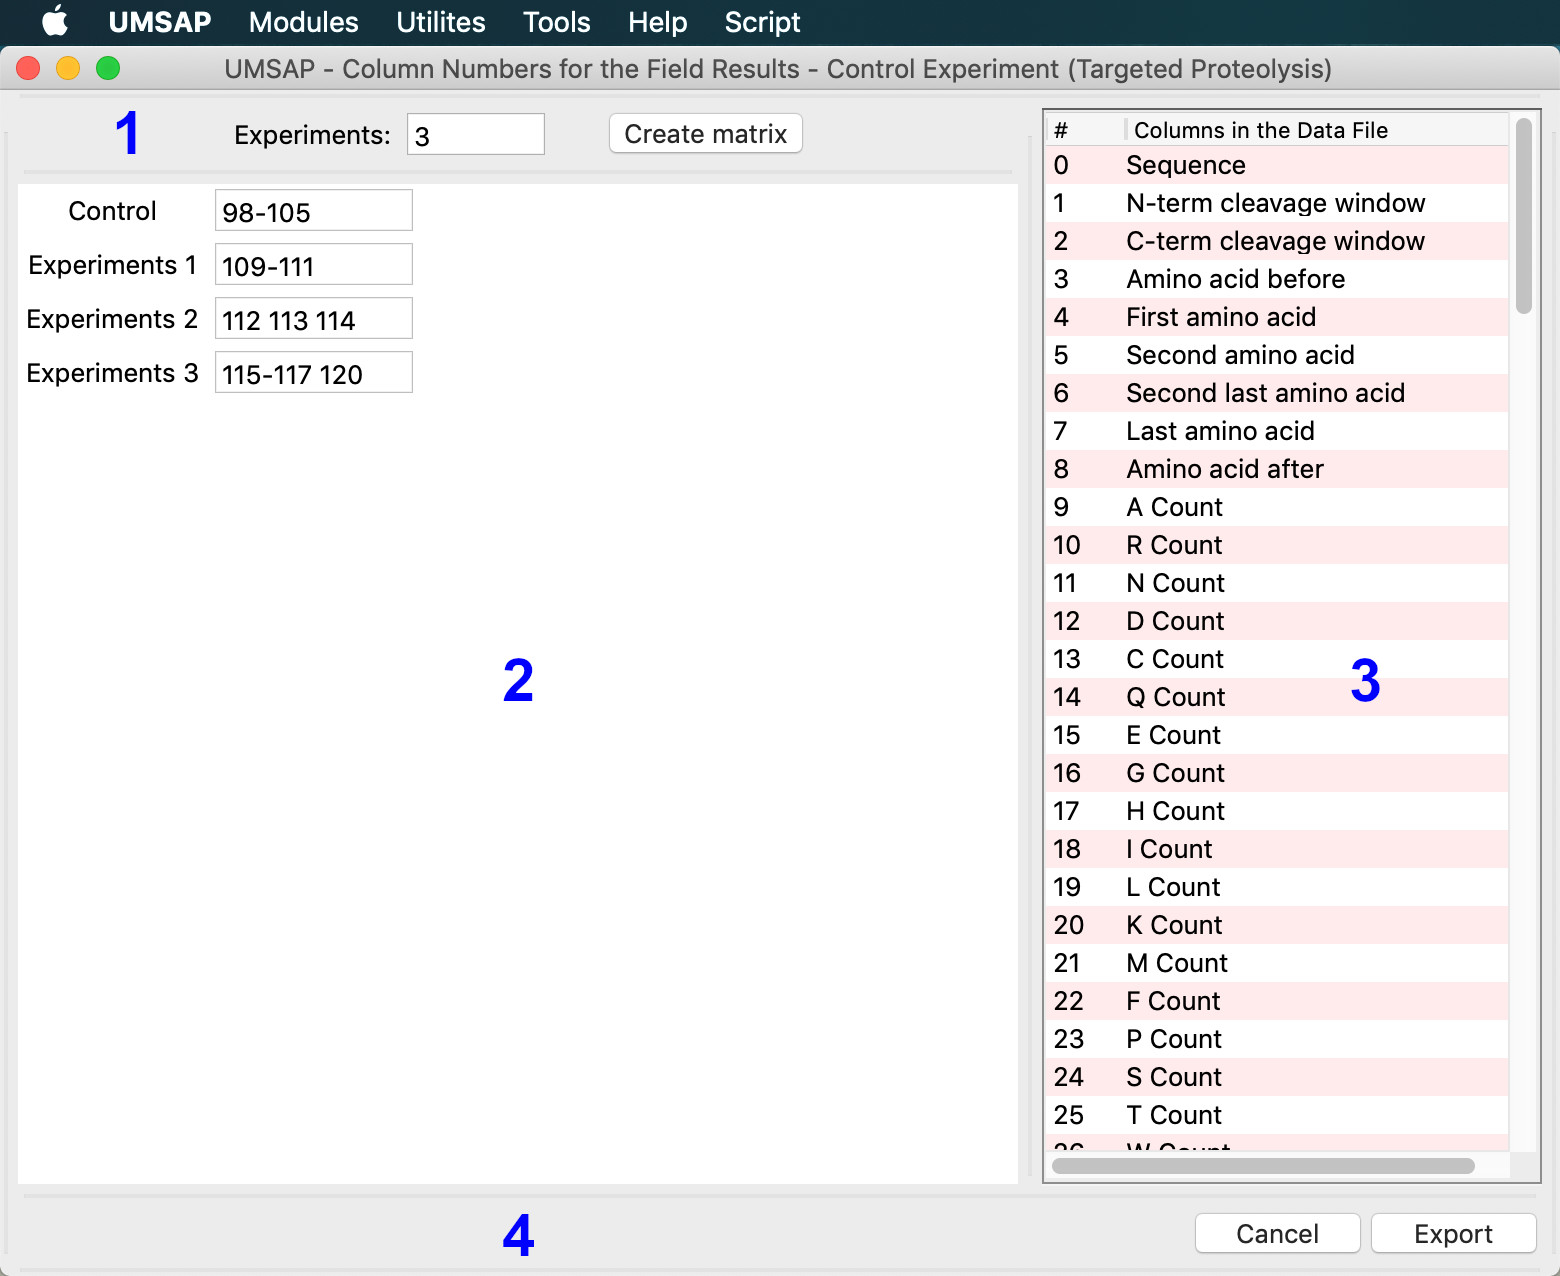
\includegraphics[width=0.7\textwidth]{./IMAGES/MOD-TARPROT/tarprot-rescontrol.jpg}
    \caption[The Result - Control experiments helper window]{\textbf{The Result -
    Control experiments helper window.} This window allows specifying the column
    numbers in the Data file containing the MS results for the selected experiments
    and control.}
    \label{fig:tarprotResControlWindow}
    \vspace{-5pt}
\end{figure}

The helper window is divided in two Regions. Region Data File Content will show the
number and name of the columns present in the selected Data file. Region
Configuration Options has two sections. The upper section allows defining the number
of experiments performed as well as the label for the control and experiments. The
button Setup Fields creates the corresponding text fields in the bottom section to
type the column numbers. Each text field should contain the column numbers with the
MS results for the given experiment. The values for the text fields should be positive
integer numbers or a range of integers, e.g. \numrange[range-phrase=--]{60}{62}.
Selected rows in the table can be copied (Cmd+C) and then pasted (Cmd+V) in the text
fields. Duplicate column numbers are not allowed.

\section{The analysis}

First, UMSAP will check the validity of the user-provided input and then the selected
Data file is read. The columns specified in section Column numbers are extracted
from the Data file. All other columns present in the Data file are discarded. After
this, all steps selected in the Data Preparation section are applied to the columns
specified in the text field Result - Control experiments (\autoref{chap:dataPrep}).
Then, the following actions are performed.

All rows in the Data file containing peptides that do not belong to the Target protein
are removed. Then, all rows containing peptides from the Target protein but with
Scores values lower than the user-defined Score threshold are removed. These steps
leave only relevant peptides, this means, peptides with a Score value higher than
the user defined threshold that belong to the Target protein. For each one of these
relevant peptides the selected statistic method is performed.

The t-test performed is a one-tailed test to check that intensity values in the
various experimental conditions explored are greater than the intensity values in
the control.

\phantomsection
The Slope test is a test for Homogeneity of Regression \cite{ancova}.
The test, \label{par:tarprotAncovaTest} done to identify relevant peptides with
different intensities in the control and a given experiment, is performed in three
steps. First, the intensity values for the replicates in the control and in a given
experiment are organized in two data sets as indicated in \autoref{fig:tarprotAncova}.
Each data set consist of two points. For the control data set the intensity values
in the replicates of the control experiment are allocated to both points. For the
experiment data set the intensity of the replicates in the control experiment are
allocated to the first point and the intensity values of the replicates in the given
experiment are allocated to the second point. The second step is to find the slope
of the straight line best fitting each data set. The third step is to test the
Homogeneity of Regression. Peptides that fail this test are included in the list of
filtered peptides (FP) because the slopes of the straight lines fitting the data
sets are significantly different at the chosen significance level. The fact that
the slopes are different implies that the peptide is found in an increased
concentration in the given experiment than in the control experiment. Only positive
slopes are considered. Peptides that past this test are not included in the list of
FP for the given experiment.

\begin{figure}[h]
    \centering
    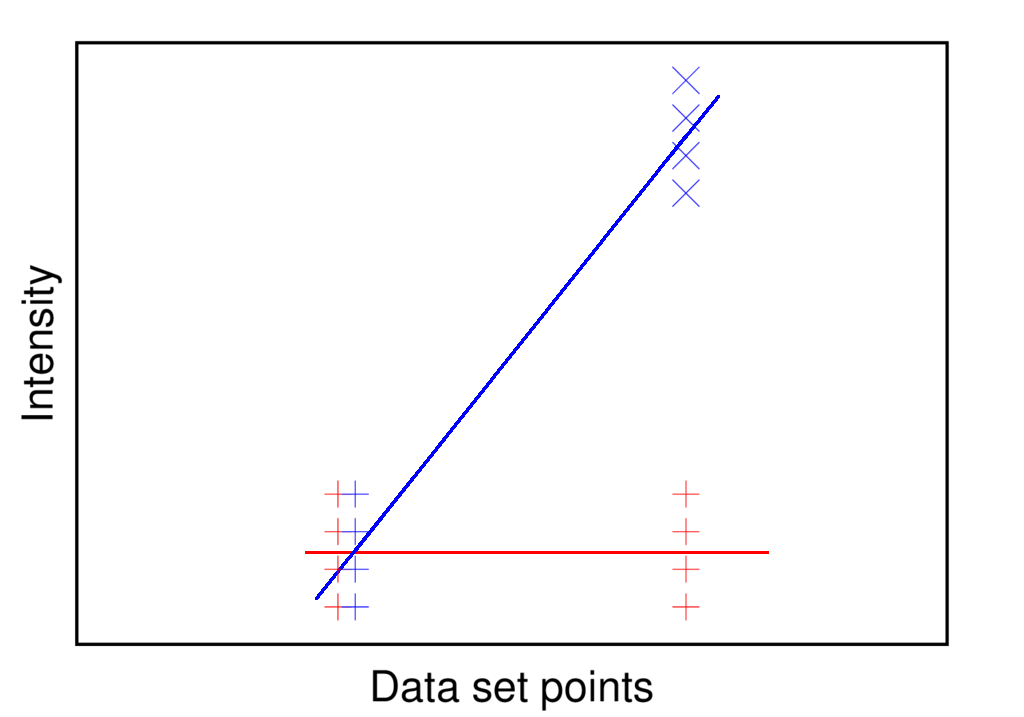
\includegraphics[width=0.7\textwidth]{./IMAGES/MOD-TARPROT/tarprot-ancova.png}
    \caption[Data organization prior to the Homogeneity of Regression test]{\textbf{Data
    organization prior to the Homogeneity of Regression test.} Two data sets with
    two points each are created, one data set for the control (red) and one for a
    given experiment (blue). The intensity data in the replicates of the control is
    used in both data points for the control (+) and in the first data point of the
    given experiment. The intensity data in the replicates of the given experiment
    is used for the second point of the data set for the given experiment (x). After
    this, the best fitting line for each data set is found and the slopes of the
    lines are compared in a test for Homogeneity of Regression.}
    \label{fig:tarprotAncova}
    \vspace{-5pt}
\end{figure}

\section{The results window}

The window showing the results from a Targeted Proteolysis analysis is divided in
four regions (\autoref{fig:tarprotFra}).

\begin{figure}[h]
    \centering
    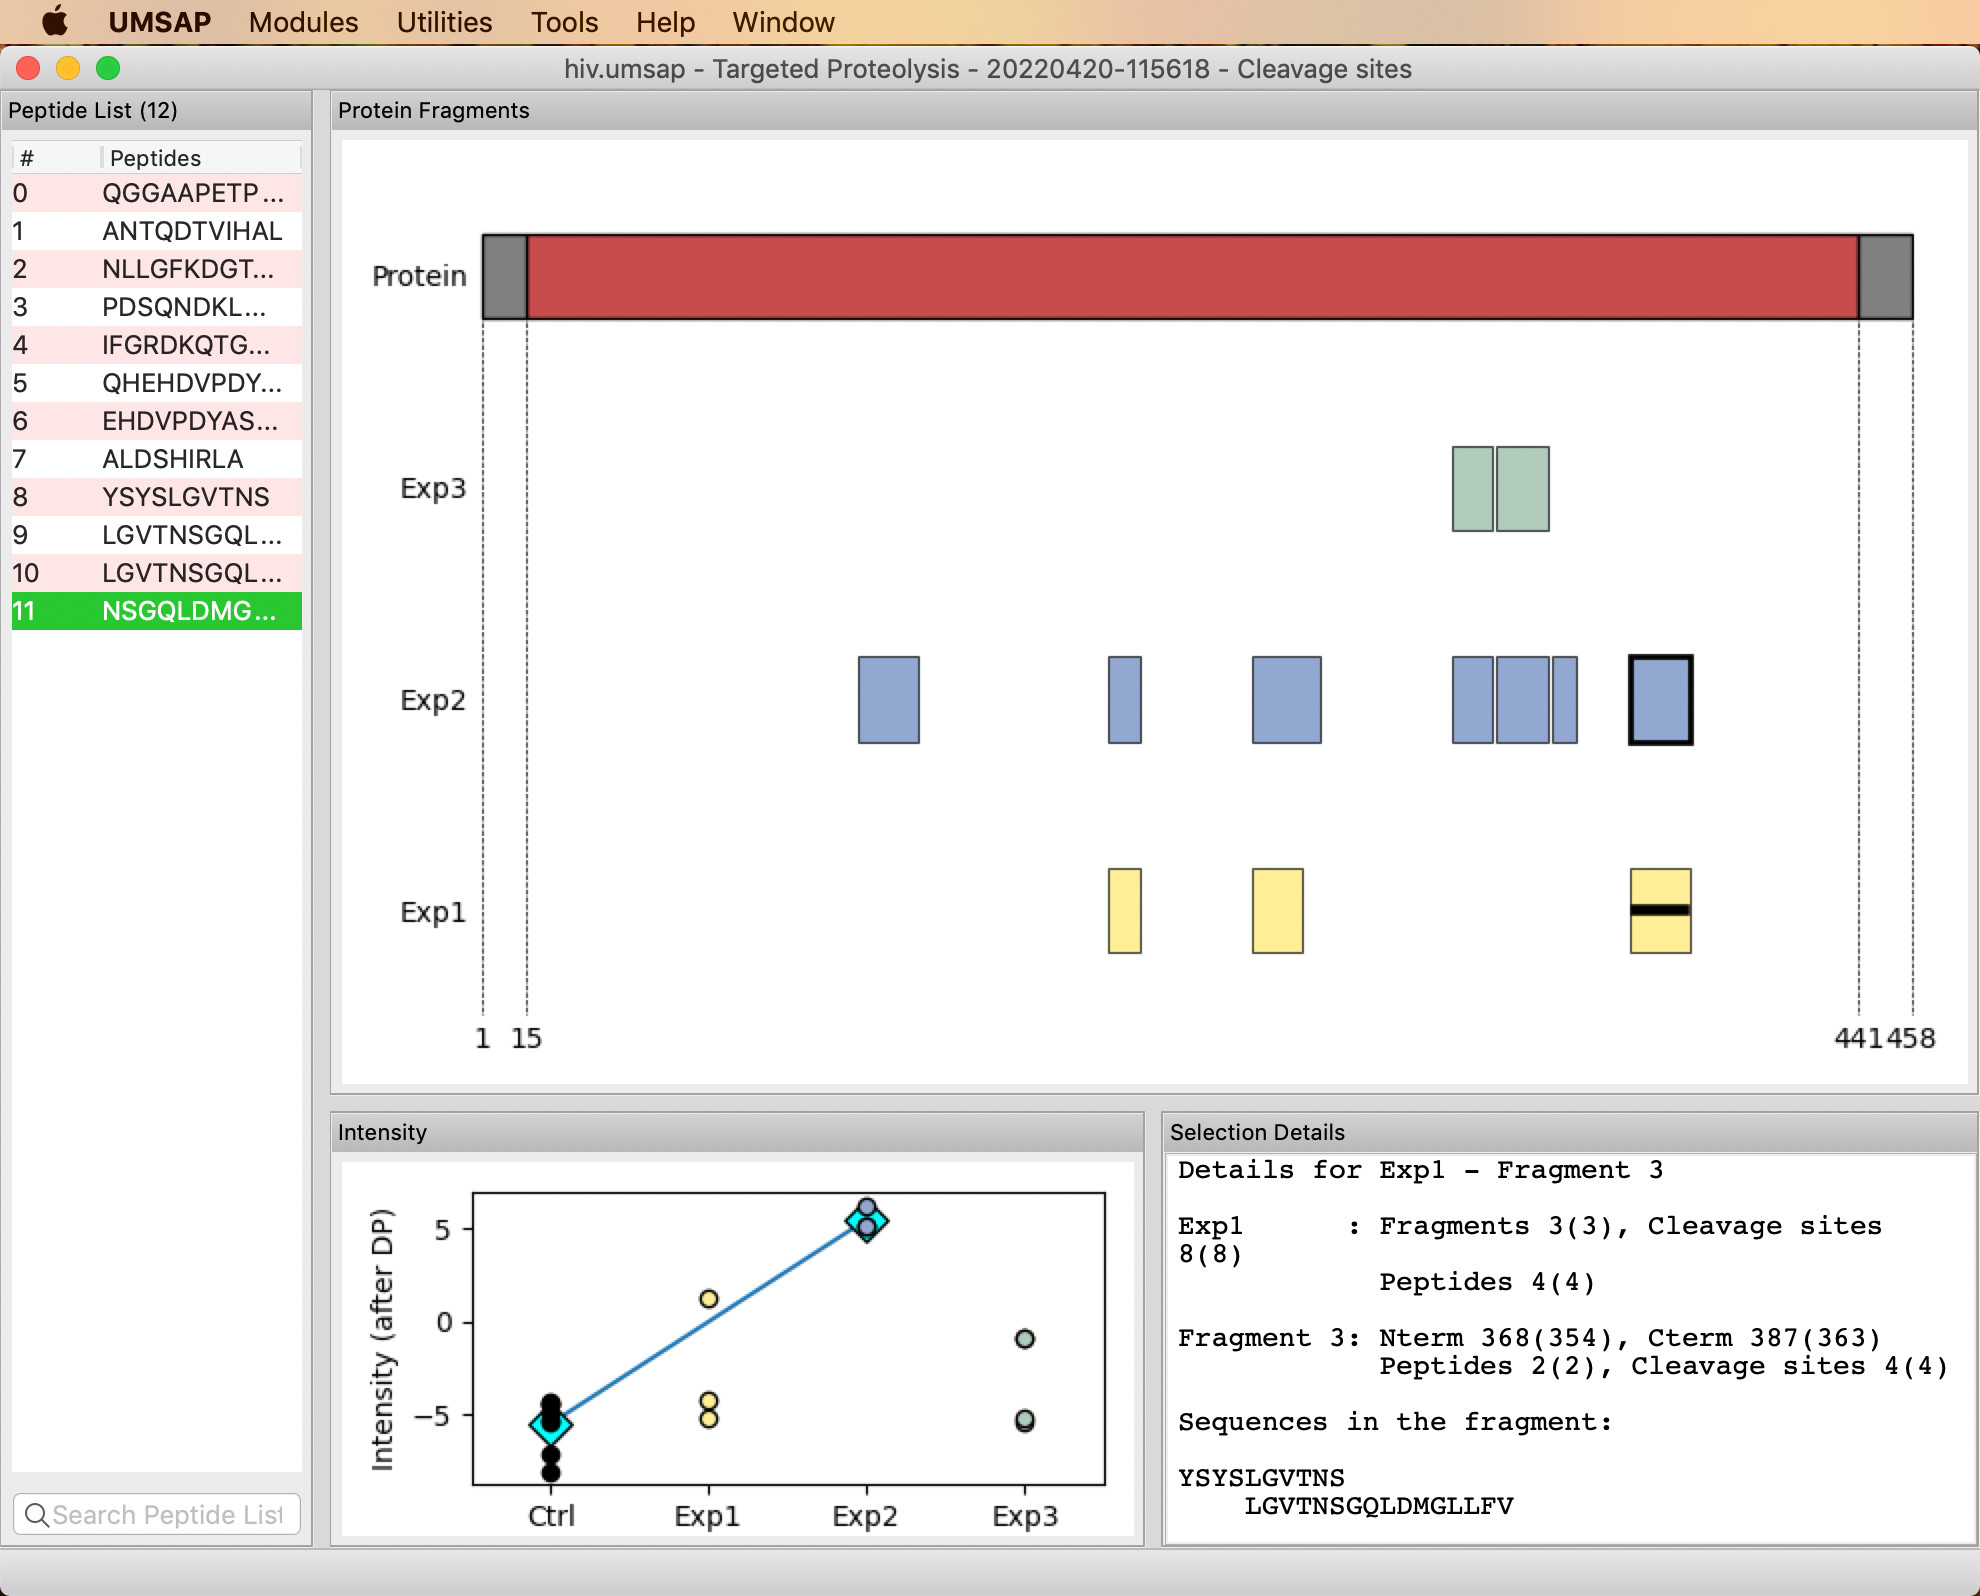
\includegraphics[width=0.8\textwidth]{./IMAGES/MOD-TARPROT/tarprot-frag.jpg}
    \caption[The Fragment analysis window]{\textbf{The Fragment analysis window.}
    Users can perform here the analysis of the fragments obtained in the enzymatic
    proteolysis experiments.}
    \label{fig:tarprotFra}
    \vspace{-5pt}
\end{figure}

Region Peptide List contains a table with all FP detected during the analysis. Selecting
a peptide in the table will highlight with a thick black border all fragments in
region Protein Fragments where the selected peptide was found. In addition, region
Intensity will show the behavior of the intensity values in the control and experiments
for the selected peptide. The search box at the bottom allows searching for a sequence
in the table of FP.

Region Protein Fragments will display a graphical representation of the fragments
found in each experiment. The first fragment in this region represents the full length
of the recombinant sequence of the Target protein. Here the central red section represents
the sequence in the recombinant protein that is identical to the native protein sequence
while gray sections represent the sequences in the recombinant protein that are different
to the native protein sequence. If the sequence of the native protein was not given
then the fragment is shown in gray. Selecting a fragment will update the information
shown in regions Selection Details.

Region Intensity will display a plot of Intensities vs experiment label. The plot
will display the data for a single peptide selected in the table of region Peptide
List. The intensity values in the plot are the ones obtained after applying the Data
Preparation workflow specified for the analysis. The values for replicates are shown
as circles. The average for a given experiment is shown as bigger cyan diamonds.
The blue lines only connect the control experiment to experiments showing intensity
values significantly higher at the chosen significance level.

Region Selection Details will display detailed information about a selected fragment
in Region Protein Fragments. In this Region regular numbers refer to the Recombinant
protein sequence while number between parenthesis refers to the Native sequence.
The Experiment section in the text contain information about the experiment in which
the fragment was identified. The information includes the total number of fragments,
the total number of sequences and the total number of unique cleavage sites identified
in the experiment. The Fragment section in the text gives similar information about
the selected fragment and also includes the first and last residue numbers in the
fragment. The rest of the lines show a sequence alignment of all the peptides in
the fragment.

\section{The Tools menu}

The menu Tools in the window showing the results from a Targeted Proteolysis analysis
allows viewing any of the analyses contained in the selected umsap file. The
submenus Fragments and Intensities allow resetting the zoom level and creating an image
of the corresponding plots.

The submenu Clear Selection allows removing any selection done by the user. In
particular, the entry All (Cmd+K) will remove all selections basically resetting
the state of the window.

The menu Tools also allows duplicating the window (Cmd+D) for easier comparison of
two or more analysis, checking the Data Preparation steps of the analysis (Cmd+P),
exporting the results of the analysis to a tab separated CSV file (Cmd+E) and to
export the sequence alignments (Cmd+S) between the peptides found in the analysis
and the sequence of the recombinant protein. In addition, the zoom level in the plots
can be reset (Shift+Alt+Z) and an image of the plots can be created (Shift+Alt+I).

The submenu Further Analysis give access to other analysis that can be performed
with the information obtained with the Targeted Proteolysis analysis.

\subsection{AA Distribution}
\label{subsec:tarprotAA}
The AA Distribution analysis allows calculating the AA distribution around
the detected cleavage sites in a Targeted Proteolysis analysis. The submenu AA Distribution
gives access to all AA distribution analyses associated with the currently selected
Targeted Proteolysis analysis. The submenu is one of the entries in submenu Further
Analysis of the menu Tools of the result window.

The entry New AA Analysis in submenu AA Distribution allows creating a new analysis.
The only input needed from the user is the number of AA positions around the cleavage
sites to be considered.

\textit{\textbf{\underline{The analysis}}}

First, UMSAP will check the validity of the user-provided input. For each FP found
in the current Targeted Proteolysis analysis, the sequence around the N and C terminal
ends of the peptide is analyzed up to the user-provided number of AA. For the N terminus
of the peptide the identity of residues in positions \(Pn\) to \(P1\) is inferred
from the sequence of the recombinant protein. The same is done for positions \(P1'\)
to \(Pn'\) at the C terminus of the peptide. If the N or C terminus of a peptide is
the first or last residue of the recombinant protein under study the N or C terminus
is excluded from the analysis. Then, the number of times that each AA
appears at a given position are counted. Finally, the absolute numbers of AA appearances
for each position are converted to percent taking the total for each position as the
sum of all counted AA in the position.

In addition, UMSAP tests whether the obtained AA distribution is significantly different
to the expected AA distribution from the proteolysis of the Target protein by a
totally non-selective protease. The first step is to generate an AA distribution with
the same number of positions defined by the user. This
distribution is generated assuming that all peptidic bonds in the recombinant protein
may be cleaved by the protease with equal probability and that all peptidic bonds
will be cleaved. Here, we are also assuming that all products of cleaving all peptidic
bonds will be detected in the MS experiment. Then, UMSAP compares each position in
both distributions using a $\chi^2$ test with the same significance level given for
the Targeted Proteolysis analysis. In order to be able to perform the $\chi^2$ test,
AAs are pooled together in the same groups as described below for the color code
used in the results window.

\textit{\textbf{\underline{The results window}}}

The window showing the results from an AA Distribution analysis contains a single
plot (\autoref{fig:tarprotAARes}).

\begin{figure}[h]
    \centering
    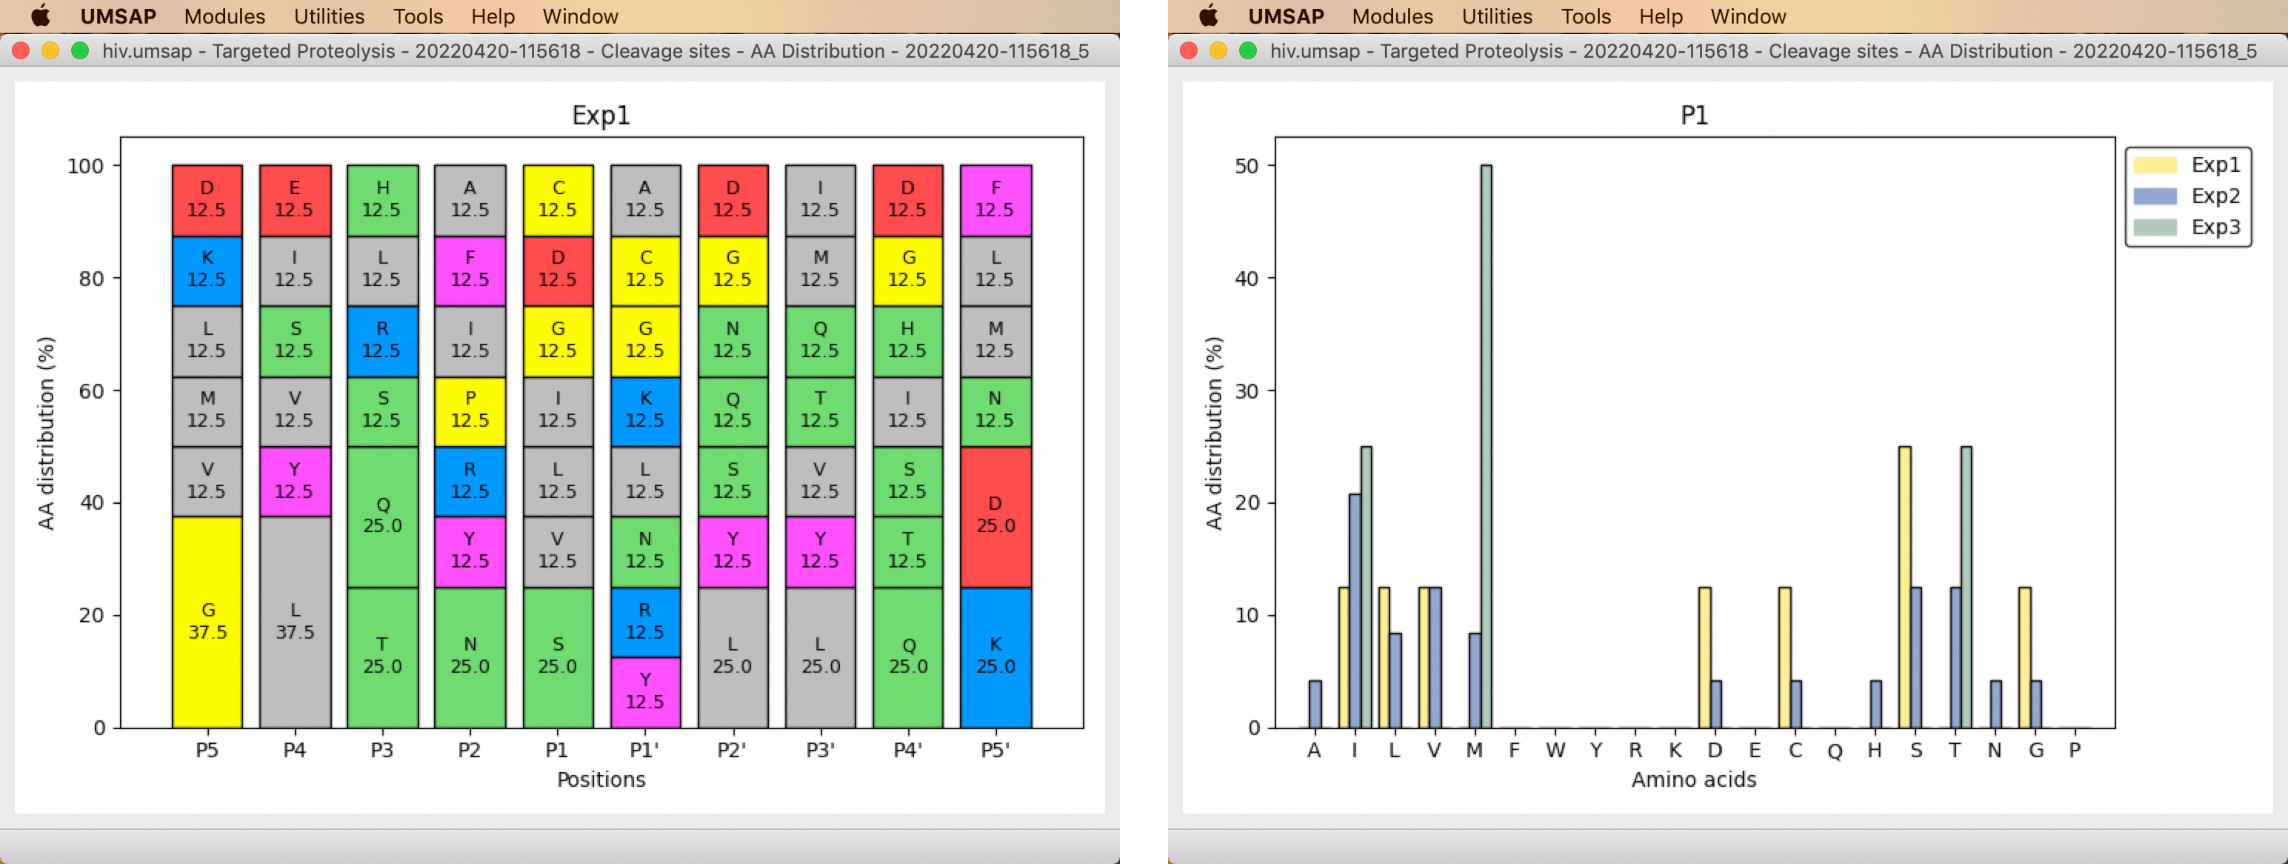
\includegraphics[width=1.0\textwidth]{./IMAGES/MOD-TARPROT/tarprot-aa.jpg}
    \caption[The AA Distribution result window]{\textbf{The AA Distribution result
    window.} This window allows visualizing the results from an AA Distribution
    analysis. The results for a given experiment (left) or position (right) can
    be shown.}
    \label{fig:tarprotAARes}
    \vspace{-5pt}
\end{figure}

The plot can show the results for a given experiment in the analysis or for one of
the considered positions.
The results for each experiment is presented as a bar graph in which each bar
represents a position. AAs are color coded with positively charged
AAs (R and K) in blue, negatively charged AAs (D and E) in red, polar AAs (S, T,
N, H, C and Q) in green, non-polar AAs (A, V, I, L and M) in gray, aromatic AAs
(F, Y and W) in pink and Gly and Pro in yellow. AAs with an occurrence higher than
\SI{10}{\percent} are labeled with the one-letter code for the AA and the percentage
value. For example, in \autoref{fig:tarprotAARes} the value of \SI{25.0}{\percent}
obtained for S in position \(P1\) means that S was found in position \(P1\) in the
\SI{25.0}{\percent} of the total cleavage sites detected.

The results of the $\chi^2$ test are given in the color of the name of the positions.
A green color represents that the obtained distribution in the position is significantly
different to a no selectivity distribution at the level of significance given for
the Targeted Proteolysis analysis. A red color represents that the distributions are
not significantly different at the level of significance given for the Targeted
Proteolysis analysis. Finally, a black color indicates that the number of expected
values below 5 was higher than the \SI{20}{\percent} threshold recommended by Yates
et al. and the test was not performed \cite{Yates1999}.

If the mouse pointer is placed on top of the bars, then information related to the
bar and the AA will be shown in the status bar at the bottom of the window. The
information includes the Position (Pos), the amino acid (AA), how many times does
the AA appear in the position as a percent of the total AA count for the given position
(\%) and the absolute number (Abs) and how many times does the AA appear in the sequence
of the recombinant protein (InSeq).

The results for the analyzed positions allows comparing the AA distribution in one
position across all experiments. This is also a bar representation in which each
bar represents an experiment and each position an AA. Placing the mouse pointer
over a bar shows information about it. The information includes the AA (AA), the
experiment (Exp), how many times does the AA appear in the position for the given
experiment as a percent of the total AA count found at the position for the given
experiment (\%) and the absolute number (Abs) and how many times does the AA appear
in the sequence of the recombinant protein (InSeq).

\textit{\textbf{\underline{The Tools menu}}}

The menu Tools in the window allows changing the displayed experiment or selecting
the position for which results in the experiments should be compared. In addition,
users may select to duplicate the window (Cmd+D) for easier comparison of the results,
to export the data shown in the window (Cmd+E), to save a figure of the plot (Cmd+I)
and to reset zoom level of the plot (Cmd+Z).

\subsection{Cleavage Evolution}
\label{subsec:tarprotCutEvol}

The Cleavage Evolution analysis allows following the Relative Cleavage Rate (RCR)
of the detected cleavage sites during a Targeted Proteolysis analysis.

\textit{\textbf{\underline{The analysis}}}

This analysis is performed by default after the Targeted Proteolysis analysis is
finished. First, UMSAP groups all MS-detected peptides that share the same \(P1\)-\(P1'\)
bond. Subsequently, the RCR is calculated as follows. For each peptide and experiment
the average intensities are calculated. The average intensity is set to \num{0} if
the peptide was not detected in a given experiment ($p>\alpha$). All other intensity
values are then scaled to the range \numrange{1}{10}. This is done in order to make
all intensity values greater than \num{0}. Subsequently, for
each peptide the scaled average intensity ratios are calculated taking as reference the
first scaled average intensity greater than zero along the experiments for each peptide.
Finally, the RCR for a \(P1\) site at an experiment is calculated
as the sum of the intensity ratios of all peptides that share the same \(P1\)
site. A numeric example is provided below.

Let's assume the following peptides were detected in a set of experiments. They all
share the same \(P1\) site at V231.

\begin{texshade}{./TeX_files/testCutEvol.fasta}
    \residuesperline*{50}
    \shadingmode[kenny]{functional}
    \hideconsensus
\end{texshade}

The intensity values for each peptide in the three experiments performed, after scaling,
are given in \autoref{table:tarprotCutEvolAveInt}.

\begin{table}[h!]
    \centering
    \begin{tabular}{lcccccc}
        \hline
        Experiment & A & B & C & D & E & F \\
        Exp1 & 2 & 0 & 0 & 3 & 3 & 10 \\
        Exp2 & 4 & 1 & 0 & 0 & 6 & 5 \\
        Exp3 & 8 & 3 & 5 & 0 & 0 & 1 \\
        \hline
    \end{tabular}
    \caption[Scaled average intensity for the detected peptide]{\textbf{Average intensity
    for the detected peptide.}}
    \label{table:tarprotCutEvolAveInt}
\end{table}

The RCR for residue V231 is then calculated as indicated in \autoref{table:tarprotCutEvolRCR}.

\begin{table}[h!]
    \centering
    \begin{tabular}{lccccccc}
        \hline
        Experiment & A       & B       & C       & D       & E       & F          & RCR\\
        Exp1       & 2/2 = 1 & 0/1 = 0 & 0/5 = 0 & 3/3 = 1 & 3/3 = 1 & 10/10 = 1  & 4  \\
        Exp2       & 4/2 = 2 & 1/1 = 1 & 0/5 = 0 & 0/3 = 0 & 6/3 = 2 & 5/10 = 0.5 & 5.5\\
        Exp3       & 8/2 = 4 & 3/1 = 3 & 5/5 = 1 & 0/3 = 0 & 0/3 = 0 & 1/10 = 0.1 & 8.1\\
        \hline
    \end{tabular}
    \caption[Relative Cleavage Rate calculation]{\textbf{Relative Cleavage Rate
    calculation.}}
    \label{table:tarprotCutEvolRCR}
\end{table}

\textit{\textbf{\underline{The results window}}}

The results window for the Cleavage Evolution analysis is divided in two regions
(\autoref{fig:tarprotCutEvol}).

\begin{figure}[h]
    \centering
    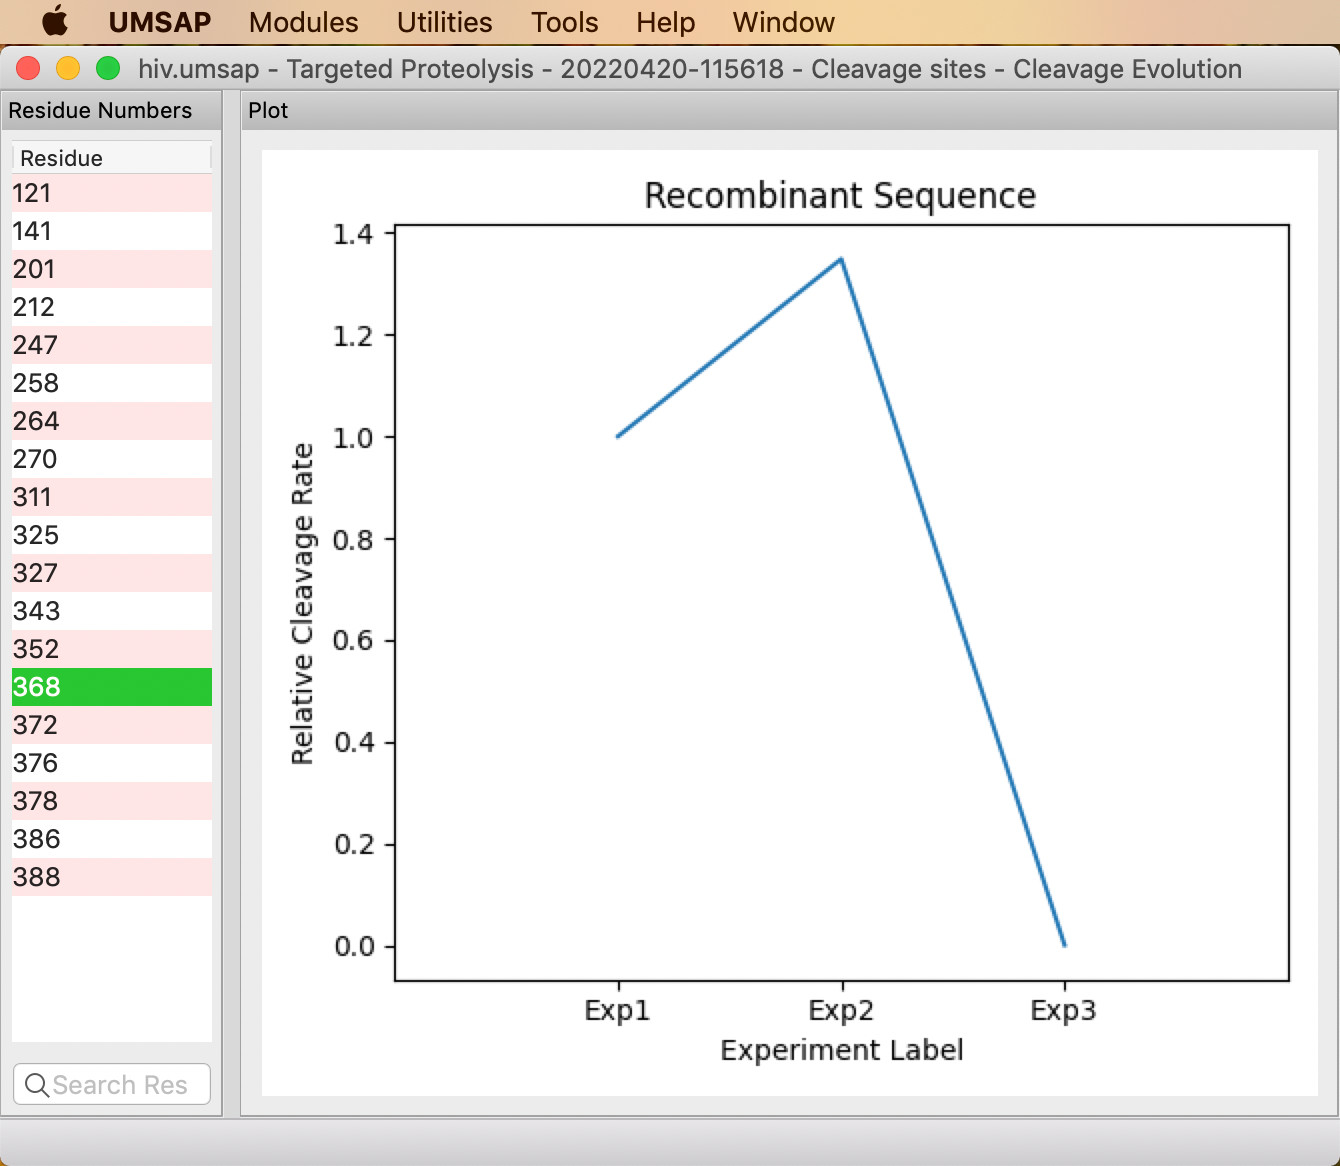
\includegraphics[width=0.7\textwidth]{./IMAGES/MOD-TARPROT/tarprot-cutevol.jpg}
    \caption[The Cleavage Evolution result window]{\textbf{The Cleavage Evolution
    result window.} This window allows visualizing the RCR for the selected Targeted
    Proteolysis analysis.}
    \label{fig:tarprotCutEvol}
    \vspace{-5pt}
\end{figure}

Region Residue Numbers shows a table with the residue numbers for which the RCR is
not zero for at least one experiment. A given residue number can be searched for using
the search box at the bottom of the table. Region Plot shows a plot of the RCR vs Experiment.
The plot can show the behavior for multiple residues selected in the table.

\textit{\textbf{\underline{The Tools menu}}}

The menu Tools allows showing the residues for the recombinant or native protein
and identifying residues whose RCR have a monotonic behavior. In addition,
users may select to duplicate the window (Cmd+D) for easier comparison of the results,
to export the data shown in the window (Cmd+E), save a figure of the plot (Cmd+I)
and to reset zoom level of the plot (Cmd+Z).

\subsection{Cleavage Histograms}
\label{subsec:tarprotHist}
The Cleavage Histogram analysis allows creating histograms of the identified cleavage
sites using the residue numbers of the Target protein as the definition of the windows
in the histograms. The submenu Cleavage Histograms gives access to all histograms
associated with the currently selected Targeted Proteolysis analysis. The submenu
is one of the entries in submenu Further Analysis of the menu Tools of the result window.

The entry New Histograms in submenu Cleavage Histograms allows creating a new histogram.
The only input needed from the user is the definition of the windows for the histograms.
Only integer numbers equal or greater than zero will be accepted as input. In addition,
the values must be organized from smaller to bigger values. Users may specify a fix
histogram window size by given just one integer number greater than zero. In this
case the histogram will have even spaced windows with the specified width. If more
than one number is provided here, then windows with the customs width will be created.
For example, the input \numlist{50 100} will create only one window
including cleavage sites between residues \numrange{50}{99}. The input
\numlist{50 100 150 200} will create three windows including cleavages sites between
residues \numrange{50}{99}, \numrange{100}{149} and \numrange{150}{199}. Duplicate values
are not allowed.

\textit{\textbf{\underline{The analysis}}}

First, UMSAP will check the validity of the user-provided input. After this, the
windows of the histograms will be created and for each experiment in the currently
selected analysis the detected cleavage sites will be assigned to the corresponding
windows. Histograms are created for the residue numbers in the recombinant protein
and for the residue numbers in the native protein if the native sequence was given
when configuring the Targeted Proteolysis analysis.

\textit{\textbf{\underline{The results window}}}

The Histograms window will display a bar plot with the selected histogram
(\autoref{fig:tarprotHistRes}).

\begin{figure}[h]
    \centering
    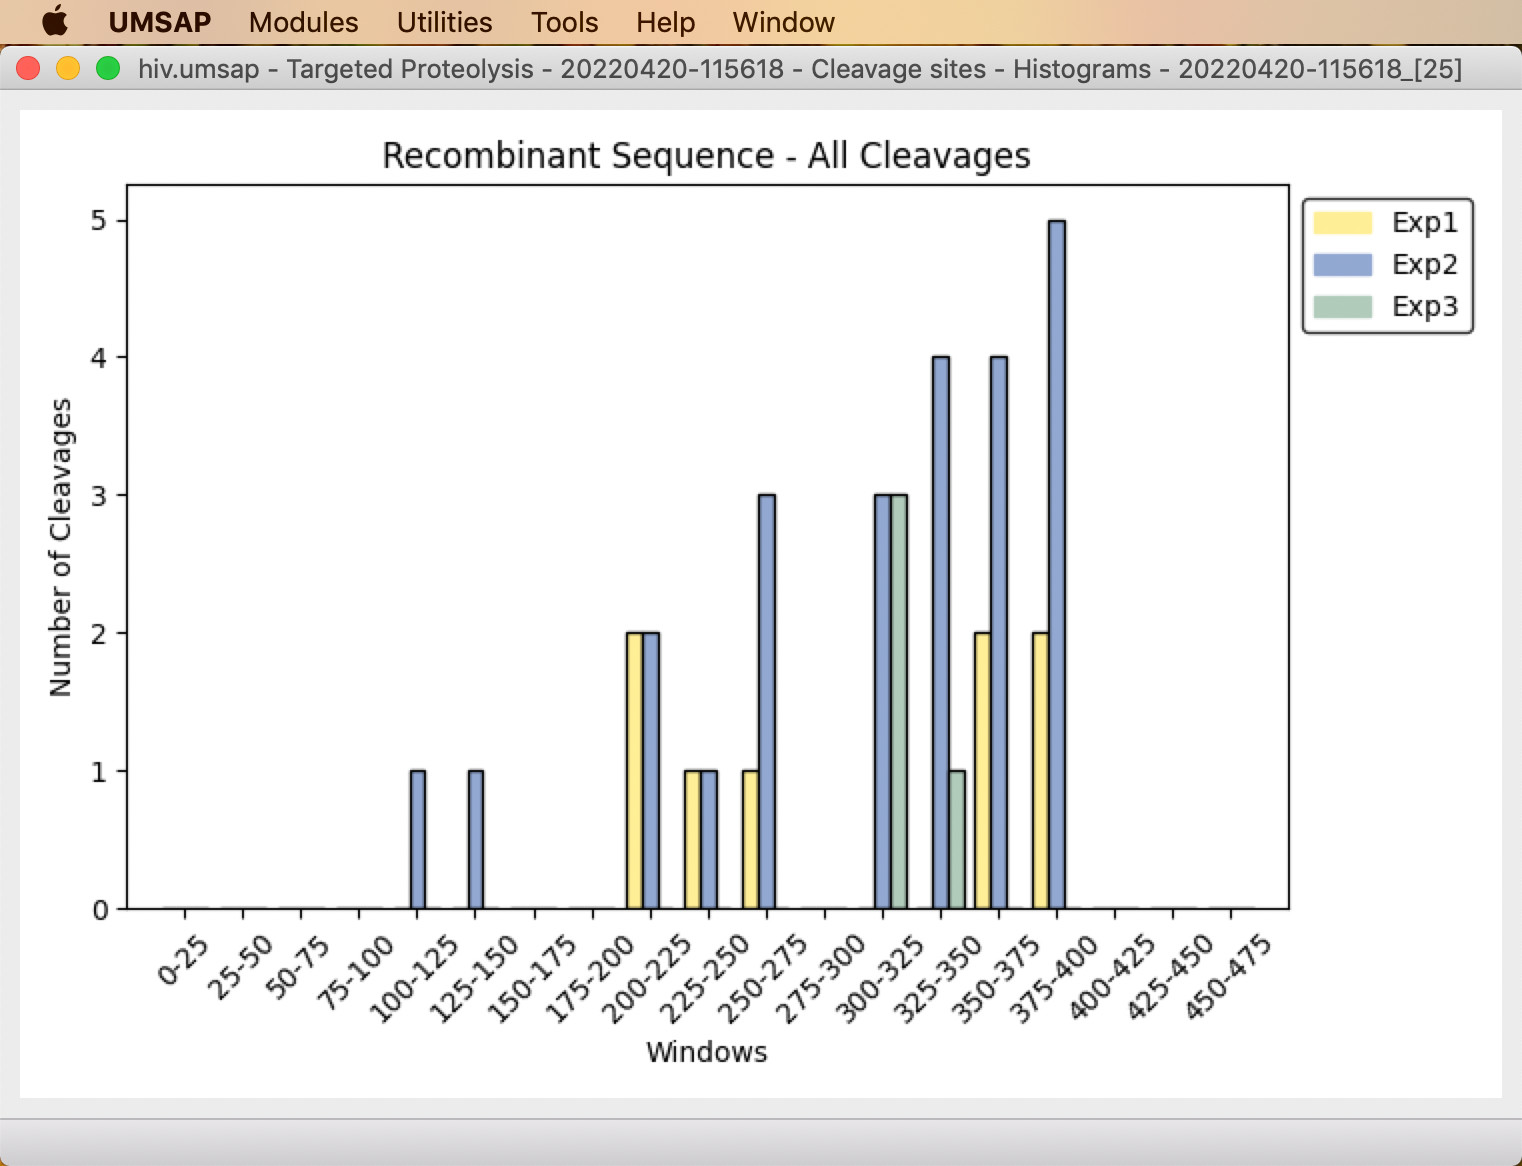
\includegraphics[width=0.7\textwidth]{./IMAGES/MOD-TARPROT/tarprot-hist.jpg}
    \caption[The Histograms result window]{\textbf{The Histograms result window.}
    This window allows visualizing the histograms generated for the selected Targeted
    Proteolysis analysis.}
    \label{fig:tarprotHistRes}
    \vspace{-5pt}
\end{figure}

In the histogram, experiments are shown in the order specified when configuring the
analysis. Placing the mouse over the plot will display information at the bottom of
the window. The information displayed includes the selected window (Win), the experiment
represented by the bar (Exp) and the number of cleavages (Cleavages).

\textit{\textbf{\underline{The Tools menu}}}

The menu Tools allows showing the results for the recombinant or native sequence and
showing only unique cleavages or the total count of the detected cleavages. In addition,
users may select to duplicate the window (Cmd+D) for easier comparison of the results,
to export the data shown in the window (Cmd+E), save a figure of the plot (Cmd+I)
and to reset zoom level of the plot (Cmd+Z).

\subsection{Cleavage per Residue}
\label{subsec:tarprotCutsRes}
The Cleavages per Residue analysis calculates the absolute number of cleavages detected
in the MS experiments for each residue in the recombinant protein under study.

\textit{\textbf{\underline{The analysis}}}

This analysis is performed by default after the Targeted Proteolysis analysis is
finished. Basically, UMSAP will count how many times each residue in the protein
under study appears at the C terminus of a FP or at the \(N-1\) position of a FP
(\(N\) is the N terminus of the FP). The cleavages per residue value for the first
and last residue of the protein under study is of course zero. This is done for
every experiment in the analysis.

\textit{\textbf{\underline{The results window}}}

The Cleavage per Residue window will display a line plot for the selected experiments
(\autoref{fig:tarprotCutsRes}).

\begin{figure}[h]
    \centering
    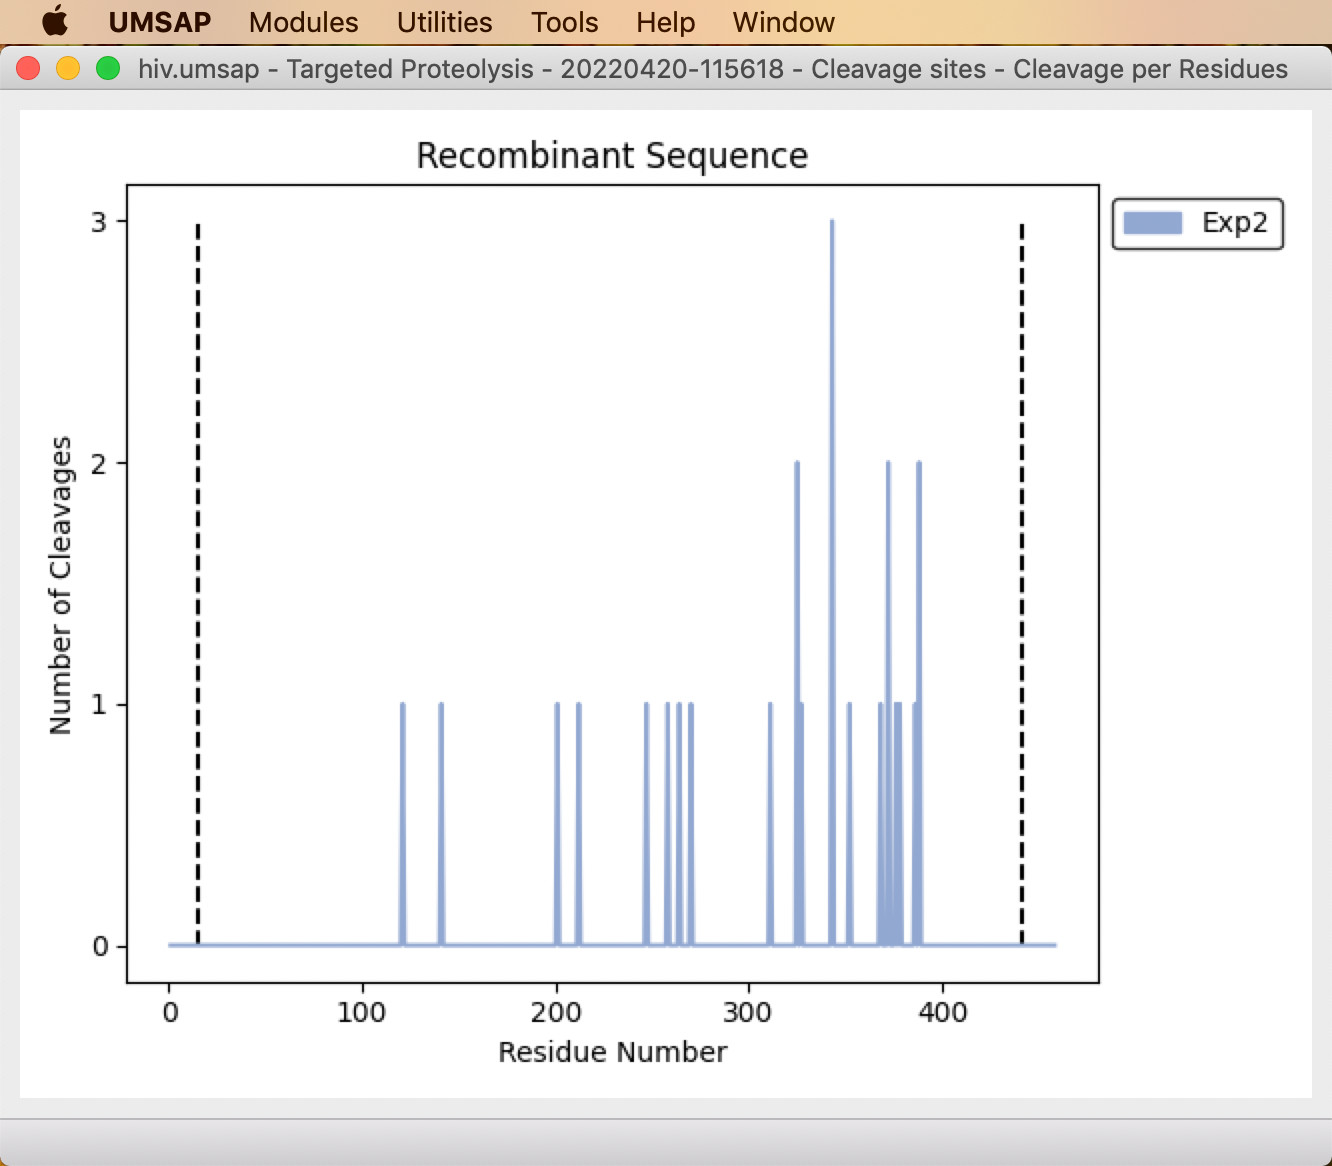
\includegraphics[width=0.7\textwidth]{./IMAGES/MOD-TARPROT/tarprot-cutres.jpg}
    \caption[The Cleavages per Residue result window]{\textbf{The Cleavages per
    Residue result window.} This window allows visualizing the cleavage per residue
    for a Targeted Proteolysis analysis.}
    \label{fig:tarprotCutsRes}
    \vspace{-5pt}
\end{figure}

The plot will be shown as a simple number of cleavages vs residue number line.
Placing the mouse pointer inside the plot will display the residue number and the
number of cleavages in the status bar at the bottom of the window. When two or more
data sets are plotted simultaneously, the number of cleavages are given in the same
order shown by the legend in the window. The dash vertical lines enclose the native
residues.

\textit{\textbf{\underline{The Tools menu}}}

The menu Tools allows showing the results for the recombinant or native sequence,
displaying one experiment or several (Cmd+S) and show/hide the dash vertical lines
enclosing the native residues. The state of the window can be reset with the Clear All
option (Cmd+K). In addition, users may select to duplicate the window (Cmd+D) for
easier comparison of the results, to export the data shown in the window (Cmd+E),
save a figure of the plot (Cmd+I) and to reset the zoom level of the plot (Cmd+Z).

\subsection{PDB Mapping}
\label{subsec:tarprotPDB}

The PDB Mapping utility maps the number of cleavages per residue found in a Targeted
Proteolysis analysis to a PDB file containing the structure of the Target protein.
The menu entry PDB Mapping is one of the entries in submenu Further Analysis of the
menu Tools in the Targeted Proteolysis result window. The only input needed from
the user are the paths to the PDB file and the folder in which the generated PDB
files will be saved. Importantly, the mapping is performed using the first chain
in the given PDB file.

\textit{\textbf{\underline{The analysis}}}

First, UMSAP will check the validity of the user-provided input. Then, a sequence
alignment between the first chain in the selected PDB file and the recombinant
sequence of the Target protein is done. Finally, the number of cleavages found in
the Cleavage per Residue and Cleavage Evolution analysis are mapped to the
corresponding residues in the PDB file. The mapping is done to the beta field of
the PDB.

\textit{\textbf{\underline{The output}}}

The output from this utility is a series of PDB files that will be saved in the
selected folder. Each file contains the number of cleavages mapped to the beta field
of the corresponding residue in the PDB structure. The results for each experiment
are mapped to individual files.




